% Chapter 1

\chapter{Introducción general} % Main chapter title

\label{Chapter1} % For referencing the chapter elsewhere, use \ref{Chapter1} 
\label{IntroGeneral}

%----------------------------------------------------------------------------------------

% Define some commands to keep the formatting separated from the content 
\newcommand{\keyword}[1]{\textbf{#1}}
\newcommand{\tabhead}[1]{\textbf{#1}}
\newcommand{\code}[1]{\texttt{#1}}
\newcommand{\file}[1]{\texttt{\bfseries#1}}
\newcommand{\option}[1]{\texttt{\itshape#1}}
\newcommand{\grados}{$^{\circ}$}

%----------------------------------------------------------------------------------------

%\section{Introducción}

%----------------------------------------------------------------------------------------
\section{Deteccion facial}
La vision artificial es un campo cientifico interdisciplinario que se encarga de como los sistemas computacionales pueden obtener un entendimiento de alto nivel de imagenes y videos digitales, para comprender y automatizar tareas como lo haria un sistema de vision humano. Las tareas que ejecuta un sistema de vision artificial son de adquisicion, procesamiento, analisis y entendimiento de imagenes. Un sistema de vision artificial esta compuesto de los siguientes elementos.

% hablar de los campos de estudio %

Uno de los campos de estudio mas importantes de la vision artificial es la deteccion facial. La deteccion facial puede ser considerada como un caso particular de la deteccion de objetos y tiene los objetivos de detectar y localizar todos los rostros humanos contenidos en una imagen digital. En la figura ...

% poner imagen %

Hoy en dia, muchos dispositivos comerciales y profesionales como smartphones, tablets y robots, utilizan la deteccion facial como primer paso para otro tipo de aplicaciones mas complejas, entre las que destacan:
- reconocimiento facial,
- computacion afectiva,
- grabacion de video inteligente

%----------------------------------------------------------------------------------------
\section{Inteligencia Artificial, Aprendizaje Automatico y Aprendizaje Profundo}

AI (\textit{Artificial Intelligence}, Intelegencia Artificial), ML (\textit{Machine Learning}, Aprendizaje Automatico) y DL (\textit{Deep Learning}, Aprendizaje Profundo), son terminos muy utilizados hoy en dia en el mundo del desarrollo tecnologico [ref]. Aunque estos terminos son muy parecidos, entre ellos existen diferencias que pueden ser visulizadas con ayuda de la figura \ref{fig:ai_ml_dl}.

\begin{figure}[h]
	\centering
	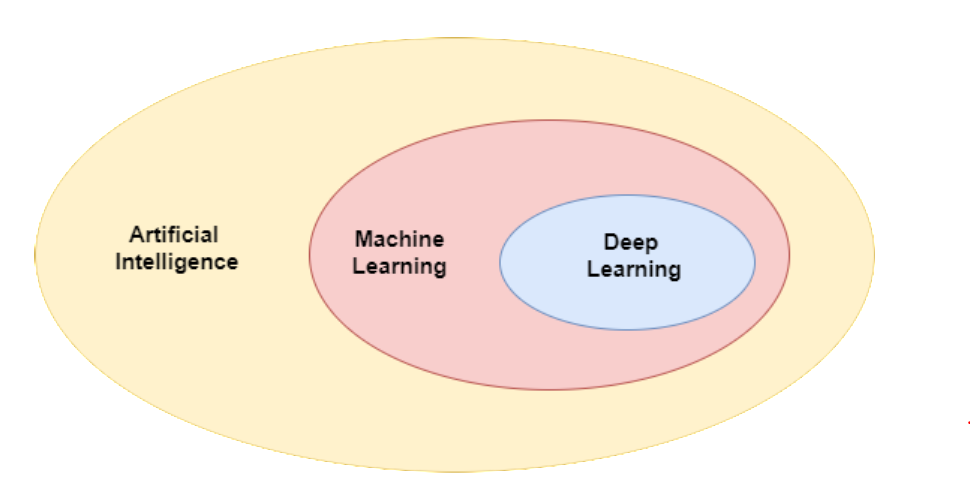
\includegraphics[scale=0.55]{./Figures/ai_ml_dl.png}
	\caption{Diferencias entre AI, ML,y DL.}
	\label{fig:ai_ml_dl}
\end{figure}

\subsection{Inteligencia Artificial}
La intelegencia artificial hace referencia a sistemas computacionales que pueden imitar la inteligencia humana para la resolucion de tareas, y pueden 

\section{Redes neuronales convolucionales}

%----------------------------------------------------------------------------------------
\section{Servicios en la nube}
El termino servicios en la nube hace referencia a un amplio rango de servicios ofrecidos bajo demanda a companias y usuarios a traves de internet. Estos servicios estan disenados para proveer de una manera facil y asequible acceso a aplicaciones y recursos, sin la necesidad de una infrastructura o hardware propios.

Los servicios en la nube son administrados totalmente por proveedores de computacion en la nube [ref]. Estos se encuentran disponibles para los usuarios desde los servidores de los proveedores, por lo que no es necesario que una empresa aloje aplicaciones en sus propios servidores.

De manera general, existen tres tipos basicos de servicios en la nube [ref]:

\begin{itemize}
	\item SaaS (\textit{Software as a Service}, Software como un Servicio): en este servicio el proveedor solo proporciona el software o aplicaciones en la nube mediante internet. Los clientes tienen acceso a traves de APIs (\textit{Application Programming Interface}, Interfaz de Programacion de Aplicaciones) o a traves de la web, que les permite interactuar de manera sencilla, sin la necesidad de gestionar, instalar ni actulizar el software. 
	\item IaaS (\textit{Infrastructure as a Service}, Infrastructura como un Servicio): este servicio implica la contatacion de una infraestructura de hardware a un tercero, donde varios cliente comparten los recursos de una maquina fisica. El proveedor proporciona a sus clientes el acceso a los recursos computacionales necesarios para almancenar o ejecutar tareas que pueden incluir servidores, redes, \textit{backup}, \textit{firewalls}, entre otros.
	\item PaaS (\textit{Platform as a Service}, Plataforma como un Servicio): es un servicio que se encuentra conceptualmente entre SaaS e IaaS al eliminar la parte fisica de la infraestructura y ofrece una plataforma donde los cliente pueden crear, desarrollar, gestionar y distribuir sus aplicaciones. El proveedor es el encargado de la gestion y mantenimiento de la plataforma y permite que los clientes se dediquen exclusivamente en el desarrollo.
\end{itemize}

En la figura \ref{fig:cloud_services} se puede observar las diferencias entre estos servicios en funcion de los elementos que pueden gestionar.

\begin{figure}[h]
	\centering
	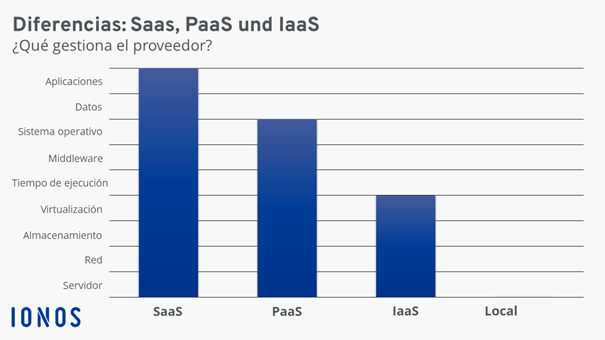
\includegraphics[scale=0.55]{./Figures/cloud_services.png}
	\caption{Capacidades de SaaS, IaaS y PaaS\protect\footnotemark.}
	\label{fig:cloud_services}
\end{figure}
\footnotetext{Imagen tomada de: \url{https://expansionba.com.ar/2020/05/23/medidas-para-amortiguar-el-costo-energetico-en-pymes/}}


%----------------------------------------------------------------------------------------
\section{Motivacion}


%----------------------------------------------------------------------------------------
\section{Estado del arte}

%----------------------------------------------------------------------------------------
\section{Objetivos y alcance}
El objetivo principal de este trabajo fue desarrollar un sistema embebido con la capacidad de ejecutar modelos de AI para detectar y localizar rostros humanos de imagenes digitales capturadas por su camara.

El alcance de este trabajo incluyo:
\begin{itemize}
	\item Construccion de un prototipo de pruebas
	\item Desarrollo e implementacion de los modelos de AI necesarios
	\item Implementacion de los servicios en la nube necesarios
\end{itemize}
%----------------------------------------------------------------------------------------
\section{Requerimientos}



%----------------------------------------------------------------------------------------
